\section{The Four Single Runs in Detail}
\label{app:single}

This appendix keeps the preprint's analysis of the four-arm ablation on
\mGLM{}, \mDS{}, \mSON{} and \mGPT{}, one run each: the full tables, the
compiled ceiling and its buckets, the clause analysis of the submitted
SQL, efficiency, and governance. The measurements stand. Its account of
\emph{why} the contract beats the manual, that the rule is one lookup away
rather than buried in a long prompt, is superseded by
Section~\ref{sec:delivery}: most of that lead was two facts the manual does
not state. Where the text below reads the clause analysis as evidence of
placement, read it as evidence that the contract arm's SQL carries facts
the manual arm was never given. The scaffolding step reported here at
$+14$ to $+15$ points on the two frontier models is not reproduced by the
repeated \mSol{} panel (Section~\ref{sec:decomposition}).

\subsection{Accuracy, the decomposition and the ceiling}
\label{app:results-k1}

\subsubsection{Accuracy and cost on four models}
\label{sec:headline}

\begin{table*}[t]
\centering
\small
\begin{tabular}{@{}lrrrr@{}}
\toprule
\tabhead{Arm} & \tabhead{Overall} & \tabhead{Hard} & \tabhead{Easy} & \tabhead{Cost} \\
\midrule
\multicolumn{5}{@{}l}{\emph{\mGLM{} (\texttt{glm-5.3-flash}, 401 tasks)}}\\
\armS{} & 22.7\% & 13.9\% & 65.2\% & \$0.76 \\
\armH{} & 26.4\% & 19.3\% & 60.9\% & \$0.85 \\
\armM{} & 31.7\% & 22.9\% & 73.9\% & \$0.96 \\
\armC{} & \textbf{57.9\%} & \textbf{55.1\%} & 71.0\% & \textbf{\$0.67} \\
\midrule
\multicolumn{5}{@{}l}{\emph{\mDS{} (\texttt{deepseek-v4-flash}, 279 tasks)}}\\
\armS{} & 33.0\% & 22.6\% & 77.4\% & \$1.79 \\
\armH{} & 31.5\% & 22.6\% & 69.8\% & \$1.52 \\
\armM{} & 52.0\% & 42.9\% & 90.6\% & \$1.69 \\
\armC{} & \textbf{61.3\%} & \textbf{56.6\%} & 81.1\% & \textbf{\$1.05} \\
\midrule
\multicolumn{5}{@{}l}{\emph{\mSON{} (Claude Sonnet~5, 401 tasks)}}\\
\armS{} & 31.9\% & 22.9\% & 75.4\% & \textbf{\$36.80} \\
\armH{} & 44.4\% & 38.0\% & 75.4\% & \$46.08 \\
\armM{} & 35.2\% & 23.8\% & 89.9\% & \$43.89 \\
\armC{} & \textbf{69.6\%} & \textbf{68.4\%} & 75.4\% & \$37.97 \\
\midrule
\multicolumn{5}{@{}l}{\emph{\mGPT{} (\texttt{gpt-5.6-sol}, 401 tasks)}}\\
\armS{} & 43.9\% & 37.0\% & 76.8\% & \$14.52 \\
\armH{} & 55.6\% & 51.2\% & 76.8\% & \$22.09 \\
\armM{} & 57.9\% & 50.3\% & 94.2\% & \textbf{\$14.42} \\
\armC{} & \textbf{78.8\%} & \textbf{77.4\%} & 85.5\% & \$21.32 \\
\bottomrule
\end{tabular}
\caption{Accuracy and cost, models in order of bare-schema capability. Hard
splits are $n{=}332$, 226, 332 and 332; easy are 69, 53, 69 and 69. \armC{}
is the most accurate arm on all four models, the cheapest on the two flash
models, and within about 3\% of the cheapest on \mSON{}. Arms are in ladder
order, so the two content-free arms are adjacent.}
\label{tab:headline}
\end{table*}

\begin{table*}[t]
\centering
\small
\setlength{\tabcolsep}{4pt}
\begin{tabular}{@{}lrrrr@{}}
\toprule
\tabhead{Comparison} & \mGLM{} & \mDS{} & \mSON{} & \mGPT{} \\
\midrule
\armS{} vs \armC{} & $3{\times}10^{-31}$ \,\, 14/\textbf{155} & $2{\times}10^{-15}$ \,\, 14/\textbf{93} & $1{\times}10^{-35}$ \,\, 11/\textbf{162} & $5{\times}10^{-32}$ \,\, 12/\textbf{152} \\
\armM{} vs \armC{} & $2{\times}10^{-17}$ \,\, 29/\textbf{134} & \textbf{0.0067} \,\, 30/\textbf{56} & $5{\times}10^{-27}$ \,\, 22/\textbf{160} & $2{\times}10^{-17}$ \,\, 12/\textbf{96} \\
\armH{} vs \armC{} & $9{\times}10^{-24}$ \,\, 23/\textbf{149} & $8{\times}10^{-17}$ \,\, 13/\textbf{96} & $2{\times}10^{-17}$ \,\, 25/\textbf{126} & $2{\times}10^{-17}$ \,\, 18/\textbf{111} \\
\armS{} vs \armM{} & $7{\times}10^{-6}$ \,\, 14/50 & $2{\times}10^{-12}$ \,\, 5/58 & \textbf{0.066} \,\, 15/28 & $2{\times}10^{-8}$ \,\, 22/78 \\
\armM{} vs \armH{} & 0.033 \,\, 55/34 & $4{\times}10^{-13}$ \,\, 63/6 & $1{\times}10^{-4}$ \,\, 27/\textbf{64} & 0.44 \,\, 58/49 \\
\armS{} vs \armH{} & \textbf{0.058} \,\, 20/35 & \textbf{0.61} \,\, 19/15 & $\mathbf{9{\times}10^{-9}}$ \,\, 14/\textbf{64} & $\mathbf{4{\times}10^{-7}}$ \,\, 20/\textbf{67} \\
\bottomrule
\end{tabular}
\caption{Every pairwise paired McNemar over all tasks: $p$-value, then
discordant pairs won by the left arm / by the right arm. The last row is the
scaffolding step of the decomposition, on which the flash and frontier
models split two and two. \mSON{}'s fourth row is its own result: the pasted
manual is not distinguishable from a bare schema.}
\label{tab:mcnemar}
\end{table*}

\armC{} wins every comparison over all tasks on all four models
(Tables~\ref{tab:headline} and~\ref{tab:mcnemar}), by 32.2, 13.7, 44.6 and
27.1 hard-task points over \armM{}. That margin is not monotone in
capability, and four points cannot support a story about why
(\appref{app:interaction}). On the two flash models \armC{} is also
the cheapest arm outright; on \mSON{} it is within about 3\% of the
cheapest; on \mGPT{} the \armM{} arm is cheaper, and
Section~\ref{sec:efficiency} says why.

Two checks tie the harness to the leaderboard. \armM{} reproduces the
published band where a comparison exists: 22.9\% hard on \mGLM{} against
the 20--26\% band for named entrants (18.8\% graded officially), and 23.8\%
on \mSON{} against the leaderboard's 19.8\% for Claude~4 Sonnet under the
same approach; on \mDS{} and \mGPT{} the same arm reaches 42.9\% and
50.3\%, above the band, which is a statement about those models. The check
is looser than it looks and in a direction that favours us, because our
grading runs 3 to 6 points high on the hard split (Section~\ref{sec:golds},
\appref{app:leniency}). The easy split is the negative check: \armC{} is not
the best arm on easy tasks on any model, and \armM{} leads on all four
(73.9\%, 90.6\%, 89.9\% and 94.2\% against 71.0\%, 81.1\%, 75.4\% and
85.5\%). The contract does nothing for questions that need no domain
knowledge, which is what it should do; an instrument that showed a contract
effect there would be measuring itself. On \mSON{} the lead is an
interaction rather than noise (62 of 69 against exactly 52 for each other
arm), and none of it is fee semantics: four of the 13 tasks involved have
their answer printed verbatim in \texttt{manual.md}, and on the rest \armC{}
returned prose the scorer cannot parse, or an ordinary near-miss.

\paragraph{On one model the manual is indistinguishable from a bare schema
on hard tasks.} \mSON{}'s \armM{} scores 79 of 332 hard tasks against
\armS{}'s 76: paired McNemar $p{=}0.72$, 17 discordant pairs one way and 14
the other. The same 24{,}177-character prompt that lifts \mGLM{} by 9 points
and \mDS{} by 20 lifts \mSON{} by less than one; the contract carrying the
same knowledge lifts it by 45.5. It is also the only model on which empty
governed tools beat the whole manual by a significant margin (38.0\%
against 23.8\%, hard split $p{=}6{\times}10^{-8}$, 15/62). One alternative is not excluded: that prompt
puts 191k input tokens per task in front of \mSON{} against \armS{}'s 91k,
and a context-load effect would produce the same null; in an independent
study, a semantic layer pasted into the prompt costs \mSON{} 11.9 points
against no layer, the largest drop of six models~\cite{evoontology}. The
clause analysis of Section~\ref{sec:clauses} cannot separate the two, since
rules absent from the SQL is what both predict.

\subsubsection{Content dominates scaffolding}
\label{app:decomposition-k1}

\begin{figure}[t]
\centering
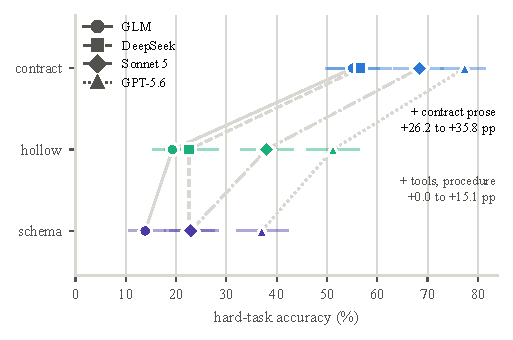
\includegraphics[width=\columnwidth]{figures/fig-ladder.pdf}
\caption{The two steps of the decomposition on hard tasks, four models in
order of bare-schema capability. Adding the nine governed tools, the
retrieval instruction, the table allow-list and the operation rules with
the prose emptied (\armS{} to \armH{}) moves accuracy by $+5.4$, $+0.0$,
$+15.1$ and $+14.2$ points; restoring the prose (\armH{} to \armC{}) moves
it by a further $+35.8$, $+34.0$, $+30.4$ and $+26.2$. Bars are Wilson
95\% intervals.}
\label{fig:ladder-single}
\end{figure}

On hard tasks the gain splits into a scaffolding step, \armS{} to \armH{},
and a content step, \armH{} to \armC{}: 13.9 to 19.3 to 55.1 on \mGLM{},
22.6 to 22.6 to 56.6 on \mDS{}, 22.9 to 38.0 to 68.4 on \mSON{}, and 37.0 to
51.2 to 77.4 on \mGPT{} (Figure~\ref{fig:ladder-single}; the same rows in
Table~\ref{tab:headline}, and the last row of Table~\ref{tab:mcnemar}).

The content step is the larger of the two on every model. The scaffolding
step depends on the model: $+5.4$ on \mGLM{} ($p{=}0.058$ over all tasks,
20/35; on the hard slice alone $p{=}0.015$), $+0.0$ on \mDS{} ($p{=}0.61$,
19/15), $+15.1$ on \mSON{} ($p{=}9{\times}10^{-9}$, 14/64) and $+14.2$ on
\mGPT{} ($p{=}4{\times}10^{-7}$, 20/67). Three of the four models favour the
scaffolding and one is flat, and the two that favour it most are from
different model families.

The claim the hollow arm was built to test survives. The sceptical reading, that
the contract helps through a narrowed table surface, an imposed procedure,
or simply by making the agent slow down, predicts that \armH{} captures most
of the gain. It does not, on any model: the content step is $6.6{\times}$
the scaffolding step on \mGLM{}, the whole of the effect on \mDS{},
$2.0{\times}$ on \mSON{} and $1.8{\times}$ on \mGPT{}. \textbf{Scaffolding is a real
but secondary effect that the content dominates everywhere.} On the two
flash models alone this step would have read as a null;
Section~\ref{sec:power} says why that would have been weak evidence.
EvoOntology credits 57\% of its evolution gain to tool edits and 34\% to
content edits~\cite{evoontology}, but its tool edits change how content
already in place reaches the agent; our scaffolding step is the tools with
the content removed.

\paragraph{Empty tools are not free.} \armH{} is the most expensive arm on
both frontier models (\$46.08 on \mSON{}, \$22.09 on \mGPT{}), makes the
most tool calls on three of the four, burns the most reasoning on \mGLM{}
and \mSON{}, and forces answers on three models where \armC{} forces none
(Table~\ref{tab:efficiency}). The transcripts show why: the agent calls
\texttt{lookup\_domain}, is told nothing is available, and searches harder.
On \mSON{} it makes that call 392 times, plus 1{,}620 calls to
\texttt{lookup\_metric} with every metric emptied; on \mGPT{}, on 401 of
401 tasks. The
models that gain most from the scaffolding are also the ones that exercise
the lookup tools hardest.

\subsubsection{The compiled ceiling and the derivation gap}
\label{app:buckets}

Every result so far compares arms to each other. None says how much of the
contract's own content an agent recovers, because nothing establishes what
recovering all of it would look like. The contract lets us establish that.
Transcribing its \texttt{sql\_expression} fields into two DuckDB views (the
fee-rule match predicate, the natural-month reconstruction, the monthly
volume and fraud-level aggregates, the fee formula, and the sum over matched
transaction--rule pairs) gives a pre-computed fee layer of the kind a
context-layer product ships. Nothing in it is authored independently of the
contract; the only work the transcription adds is composition.

Which tasks the views cover is decided from question text alone, never
from gold and never from any arm's output. DABStep's tasks are instances of
parameterised question shapes (Section~\ref{sec:dabstep}), and five of
those shapes, in eleven date and grouping variants, ask exactly what the
views compute: the total fees a merchant paid in a period, the fee rules
that applied to it, the merchants a rule applies to, the average fee for a
transaction profile, and the rules matching an account type and ACI. A
regular expression per shape matches 176 of the 401 tasks, all hard.
Instantiating the views with each task's own parameters and grading the
result with the official scorer gives the ceiling: \textbf{the compiled
contract reproduces the benchmark's gold answer on every one of the 176
tasks it covers.} This is a statement about the artifact, not about an
agent, and it has two uses. It answers the objection that \armC{} wins
because the contract is subtly wrong in a benchmark-favouring way: it
compiles to gold. And it converts accuracy into recovery against a proven
ceiling. We call the 176 the \emph{macro} bucket. Of the remaining tasks,
148 need the same semantics plus a counterfactual or an optimisation the
views do not encode (\emph{derived}), and 77 involve no fee semantics. A
layer compiled from a domain contract's declared expressions therefore
reaches 53\% of this benchmark's hard set, a bound on that kind of layer
rather than on pre-computation in general (Section~\ref{sec:prior}). On
the 176, whatever an agent fails to get is a failure to derive
(Table~\ref{tab:buckets}; \appref{app:golds} says which of the 176 share a
premise with the gold verification).

\begin{table*}[t]
\centering
\small
\setlength{\tabcolsep}{4pt}
\begin{tabular}{@{}lrrrrrrrr@{}}
\toprule
& \multicolumn{2}{c}{\mGLM{}} & \multicolumn{2}{c}{\mDS{}} & \multicolumn{2}{c}{\mSON{}} & \multicolumn{2}{c}{\mGPT{}} \\
\cmidrule(lr){2-3}\cmidrule(lr){4-5}\cmidrule(lr){6-7}\cmidrule(lr){8-9}
Hard tasks & \emph{macro} & \emph{derived} & \emph{macro} & \emph{derived} & \emph{macro} & \emph{derived} & \emph{macro} & \emph{derived} \\
\midrule
\armS{} & 2.8\% & 25.0\% & 8.5\% & 34.7\% & 6.8\% & 37.8\% & 31.8\% & 41.2\% \\
\armH{} & 10.2\% & 25.7\% & 10.2\% & 31.7\% & 36.4\% & 37.2\% & 46.6\% & 54.1\% \\
\armM{} & 14.8\% & 32.4\% & 38.1\% & 44.6\% & 8.5\% & 38.5\% & 49.4\% & 48.6\% \\
\armC{} & \textbf{60.8\%} & \textbf{45.9\%} & \textbf{62.7\%} & \textbf{46.5\%} & \textbf{73.9\%} & \textbf{60.1\%} & \textbf{94.9\%} & \textbf{56.1\%} \\
\midrule
\emph{compiled contract} & \emph{100\%} & --- & \emph{100\%} & --- & \emph{100\%} & --- & \emph{100\%} & --- \\
\bottomrule
\end{tabular}
\caption{Hard tasks split by whether the compiled contract answers the task
outright (\emph{macro}, $n{=}176$; 118 on \mDS{}'s complete-case set) or
requires reasoning on top of it (\emph{derived}, $n{=}148$; 101). The gap
between \armC{} and the compiled contract on \emph{macro} is derivation
failure on information the agent provably had.}
\label{tab:buckets}
\end{table*}

Three readings follow.

\textbf{The contract's advantage concentrates where its semantics apply
directly.} Over \armS{} it is $+58.0$, $+54.2$, $+67.1$ and $+63.1$ points on
\emph{macro} against $+20.9$, $+11.8$, $+22.3$ and $+14.9$ on \emph{derived}.
This is the domain-specificity of Section~\ref{sec:domain}, measured on a
cleaner boundary.

\textbf{The two buckets do not move together.} \armC{} scores 60.8\%, 62.7\%,
73.9\% and 94.9\% on \emph{macro}, rising with capability (with one caveat:
\mDS{} and \mSON{} are 0.3 points apart on the capability axis and 11 apart
here), against 45.9\%, 46.5\%, 60.1\% and 56.1\% on \emph{derived}, which
rises under no ordering: \mSON{} leads it while trailing \mGPT{} by 21
points on \emph{macro}.

\textbf{The derivation gap closes with capability.} Read against the
ceiling, the \emph{macro} series is a shortfall of 39.2, 37.3, 26.1 and 5.1
points below an accuracy proven reachable: the \emph{derivation gap}, the
price of making an agent derive a query the contract could have
pre-computed. Against a ceiling of 100\% the gap is arithmetically the arm's
error rate, and ``errors fall as models improve'' is not a finding. The
finding is the contrast with \emph{derived}, whose shortfall we call the
\emph{composition gap}: between the flash models and the strongest one, the same capability increment closes 87\% of the
macro-bucket gap and 19\% of the derived-bucket one, and \mSON{}'s
\emph{macro} score falls between the flash models and \mGPT{} while its
\emph{derived} score exceeds all three. We recorded the direction of this
result publicly before \mGPT{} ran, predicting a \emph{macro} score ``well
above 62.7\%, moving toward 100\%'' if capability governed it and ``near
61--63\%'' if the harness did; the observed value is 94.9\%. \mSON{}, run
last and outside the prediction, lands at 73.9\%: the direction replicated,
the size did not.

This bears on the economics of Section~\ref{sec:intro}. The derivation gap
is exactly what separates a declarative contract, which requires the agent
to derive the query, from pre-computed macros, which do not. A gap fixed
near 38 points would be a standing structural cost of the declarative
approach. A gap that falls to 5 points on the strongest model is a
\emph{transient} cost, one the trend in model capability is already paying
down, while the per-metric authoring cost of a macro layer is paid down by
nothing. What survives the strongest model is not difficulty in knowing the
domain but the counterfactual and optimisation reasoning built on top of it,
on which the four models have no clean ordering.

\subsubsection{The gain stays inside the contract's domain}
\label{sec:domain}

DABStep's hard set is dominated by one question family: 294 of 332 hard
tasks concern fees, and the contract encodes fee semantics. On those 294 the
contract arm scores 59.2\%, 61.2\%, 73.5\% and 83.7\% against the manual
arm's 24.5\%, 44.9\%, 24.1\% and 53.4\%. On the 38, 30, 38 and 38 hard tasks
that do not concern fees it holds no detectable advantage (9 against 4, 8
against 9, 11 against 8 and 11 against 10 correct), and on \mGPT{} the bare
schema leads the slice outright at 14, the only slice in the four runs where
it does (\appref{app:domain}). Thirty of the 38 are one family, which needs
the fee rules without naming them and scores 0 to 3 of 30 for every arm on
three of the four models. The slices are too small to be a negative result
and equally unable to support a general claim. ``Hard accuracy'' on this
benchmark is close to ``fee-question accuracy'', so the result should be
stated as: \textbf{a contract carrying a domain's semantics produces a large
gain on questions in that domain.} That is what a domain contract should do,
and it is why this benchmark cannot answer the general question.

\subsection{What the contract arm's SQL carries}
\label{sec:why}

Aggregate accuracy does not explain itself. This section traces one task end
to end, reads the SQL every arm submitted, accounts for the work and money
each arm spent, and looks at where the contract arm still loses.

\subsubsection{The rule was in both prompts; only one arm's SQL carries it}
\label{sec:reach}
\label{sec:clauses}

Task~1278 asks for \emph{the average fee NexPay would charge for a credit
transaction of 50 EUR}.

\begin{center}
\footnotesize
\setlength{\tabcolsep}{4pt}
\begin{tabular}{@{}lr@{}}
\toprule
Gold      & \texttt{0.352294} \\
\armC{} (correct)  & \texttt{0.352294} \\
\armM{} (wrong)    & \texttt{0.353053} \\
\armS{} (wrong)    & \texttt{0.353053} \\
\midrule
\texttt{is\_credit IS NULL OR is\_credit = true} & \texttt{0.352294} \\
\texttt{is\_credit = true} & \texttt{0.353053} \\
\bottomrule
\end{tabular}
\end{center}

Both figures reproduce against the warehouse with the two predicates
shown. A \texttt{NULL} in a \texttt{fees} column means \emph{this rule
applies to every value}, not \emph{unknown}; both baselines dropped the
\texttt{NULL} rows and produced the identical wrong number. The contract arm called
\texttt{lookup\_domain("fees")}, and its recorded reasoning states the rule
back: \emph{``rules that apply to credit transactions: is\_credit true or
null''}.

The decisive detail is that \texttt{manual.md} documents this rule too.
\armM{} had it, inside a 24{,}177-character system prompt. \armC{}'s system
prompt is 2{,}475 characters, with the rule reachable by one targeted call.
Two published results frame the difference: retrieval quality falls for
material buried mid-prompt~\cite{lost-in-the-middle}, and what a tool's
documentation says changes what an agent does with
it~\cite{tool-documentation}. \armM{}'s copy of the rule was buried
mid-prompt; \armC{}'s was a tool's documentation. EvoOntology reports the
same contrast on another benchmark~\cite{evoontology}: an agent-built
semantic layer placed in the prompt scores below no layer at all on five
of six models, while the same layer served through two MCP lookup tools,
before any revision, gains 12.3 points averaged over four of them.

The finding is not that the contract arm was given more information: for
this rule both arms had it, and only one used it. What the contract changes
is where the rule sits at the moment of use, in the result of one targeted
call rather than in a long prompt. The scoping matters: it holds for the
clauses the manual states outright, which is the class this failure
belongs to, and not for the three clauses the contract resolves on its own
(Section~\ref{sec:interpretation}).

One task shows the mechanism. Whether it is general can be read from the
SQL every arm submitted, rather than from the answers. We defined one detector per clause of the contract's fee semantics
that a correct query must express: the \texttt{NULL}-wildcard disjunct, the
empty-list wildcard, the capture-delay band mapping, a per-merchant monthly
aggregate, the natural-month reconstruction, and fraud measured on euro
volume. We then restricted the comparison to the 97 tasks that require all
six (69 on \mDS{}, whose truncation cost the rest), so every row compared
carries the same requirement (Table~\ref{tab:clauses}). The detectors are
deliberately permissive: the question is whether the agent expressed the
idea, not whether it copied the contract's phrasing.

\begin{table}[t]
\centering
\footnotesize
\setlength{\tabcolsep}{3pt}
\begin{tabular}{@{}lrrrr@{}}
\toprule
\tabhead{Wrote all six clauses} & \mGLM{} & \mDS{} & \mSON{} & \mGPT{} \\
\midrule
\armS{} & 7\% & 4\% & 3\% & 8\% \\
\armH{} & 14\% & 4\% & 4\% & 8\% \\
\armM{} & 3\% & 9\% & 4\% & 4\% \\
\armC{} & \textbf{39\%} & \textbf{65\%} & \textbf{55\%} & \textbf{98\%} \\
\bottomrule
\end{tabular}
\caption{Share of the 97 tasks requiring all six fee clauses (69 on \mDS{})
on which the agent's submitted SQL expresses all six. \armM{} holds the same
knowledge as prose in its system prompt. \armC{} against \armM{} is
$p{=}2{\times}10^{-10}$, $3{\times}10^{-12}$, $9{\times}10^{-16}$ and
$2{\times}10^{-47}$ (Fisher exact).}
\label{tab:clauses}
\end{table}

\textbf{Note what does not move.} \armM{} writes no more of the contract's
clauses on a strong model than on a weak one (3\%, 9\%, 4\%, 4\%), while
\armC{} reaches 55\% and 98\% on the two frontier models. \mSON{} is the
extreme case: 4\% against 55\% in the SQL, no better than a bare schema
against 45 points above it in accuracy. Capability does not, on its own,
make a model extract structure from prose; it makes a model much better at
\emph{using} structure it is handed. That is the same asymmetry the
derivation gap shows (Section~\ref{sec:ceiling}), measured on behaviour
instead of outcomes.

\textbf{What this does not measure.} Clause presence does not predict
success: within every arm on every model, attempts that got the task right
and attempts that got it wrong write the same clauses (every Fisher
$p{\ge}0.14$), and \armH{} on \mGLM{} writes more clauses than \armM{} while
scoring at the bare-schema floor. The measure captures whether the
contract's vocabulary reaches the query, not whether the query is any good.

\subsubsection{Less work, and usually less money}
\label{sec:efficiency}
\label{app:efficiency}

\begin{table*}[t]
\centering
\small
\begin{tabular}{@{}lrrrr@{}}
\toprule
 & \armS{} & \armH{} & \armM{} & \armC{} \\
\midrule
\multicolumn{5}{@{}l}{\emph{\mGLM{}}}\\
Turns / task & 12.1 & 8.4 & 9.8 & \textbf{7.1} \\
Tool calls & 5{,}134 & 4{,}110 & 4{,}282 & \textbf{3{,}355} \\
Reasoning tokens & 428k & 525k & 400k & \textbf{154k} \\
Cost / correct & \$0.0084 & \$0.0080 & \$0.0076 & \textbf{\$0.0029} \\
Forced answers & 41 & 0 & 18 & \textbf{0} \\
\midrule
\multicolumn{5}{@{}l}{\emph{\mDS{}}}\\
Turns / task & 13.7 & 11.4 & 12.8 & \textbf{8.2} \\
Tool calls & 5{,}489 & 6{,}375 & 4{,}770 & \textbf{4{,}155} \\
Reasoning / task & 10{,}941 & 10{,}766 & 9{,}243 & \textbf{4{,}844} \\
Cost / correct & \$0.0195 & \$0.0173 & \$0.0117 & \textbf{\$0.0061} \\
Forced answers & 49 & 15 & 38 & \textbf{0} \\
\midrule
\multicolumn{5}{@{}l}{\emph{\mSON{}}}\\
Turns / task & 11.3 & 10.0 & 11.1 & \textbf{7.0} \\
Tool calls & 5{,}644 & 6{,}494 & 5{,}176 & \textbf{3{,}791} \\
Reasoning tokens & 942k & 1{,}411k & 1{,}044k & \textbf{824k} \\
Cost / correct & \$0.288 & \$0.259 & \$0.311 & \textbf{\$0.136} \\
Forced answers & 43 & 27 & 32 & \textbf{0} \\
\midrule
\multicolumn{5}{@{}l}{\emph{\mGPT{}}}\\
Turns / task & 7.9 & 10.4 & 7.6 & \textbf{6.5} \\
Tool calls & 5{,}099 & 7{,}997 & \textbf{4{,}354} & 5{,}245 \\
Reasoning tokens & 357k & 311k & 277k & \textbf{141k} \\
Cost / correct & \$0.082 & \$0.099 & \textbf{\$0.062} & \$0.067 \\
Forced answers & 0 & 8 & 0 & \textbf{0} \\
\bottomrule
\end{tabular}
\caption{Work and cost per arm. The contract arm uses the fewest turns and
the least reasoning on every model and never exhausts its output budget; it
is the cheapest arm per correct answer on three of the four. \mDS{}'s
reasoning row is per task rather than a total, because its complete-case set
has fewer rows than the other runs.}
\label{tab:efficiency}
\end{table*}

\armC{} is not thinking harder; it has less to search for. On all four
models it uses the fewest turns and the least reasoning (by a factor of two
to three on three models, by 12\% on \mSON{}), and it is the only arm that
never exhausted its output budget on any model (Table~\ref{tab:efficiency};
on reporting cost beside accuracy, see~\cite{agents-that-matter}).
EvoOntology's lookup layer cuts turns the same way, from 14.6 per task to
8.4~\cite{evoontology}.

Money follows work on three models and not on the fourth. \armC{} is the
cheapest arm outright on both flash models, and per correct answer it is the
cheapest on \mGLM{}, \mDS{} and \mSON{}, by about $2{\times}$ on \mSON{}
(\$0.136 against \$0.259 for the next arm). On \mGPT{} it bills \$21.32
against \armM{}'s \$14.42, and \$0.067 per correct answer against \$0.062.
The recorded token counts locate the difference (Table~\ref{tab:gptcost}):
fresh, uncached input accounts for \$5.3 of the \$6.9 gap and output for
\$1.6, and cached input is a wash. \armC{} reads 1{,}692 fresh tokens per
turn against \armM{}'s 582, because its knowledge arrives as tool results.
On \mGPT{} it calls \texttt{lookup\_metric} 1{,}690 times and
\texttt{lookup\_domain} 776 times over 401 tasks, two tool calls per turn,
and each result is billed at the fresh rate when it first enters the
context. \armM{}'s knowledge sits in a system prompt that is the same prefix
in every request of every task, and is billed at the cached rate. \armC{}
also emits more visible output (726k tokens against 425k) despite half the
reasoning (141k against 277k), because \mGPT{} validates before it runs: 676
\texttt{inspect\_query} calls against 622 \texttt{run\_query}, so most
queries are written twice. \mSON{} shows the same mechanism (1{,}976 against
1{,}037 fresh tokens per turn), but its \armM{} arm carries 191k tokens of
context per task and pays \$14.40 in cached input alone, which is what makes
the contract arm cheaper there.

\begin{table}[t]
\centering
\footnotesize
\setlength{\tabcolsep}{5pt}
\begin{tabular}{@{}lrrrr@{}}
\toprule
\mGPT{} & \tabhead{Fresh input} & \tabhead{Cached input} & \tabhead{Output} & \tabhead{Total} \\
\midrule
\armM{} & \$3.55 & \$3.85 & \$7.02 & \$14.42 \\
\armC{} & \$8.87 & \$3.78 & \$8.67 & \$21.32 \\
\bottomrule
\end{tabular}
\caption{\mGPT{}'s bill for the two content-bearing arms, decomposed from the
recorded token counts at the pinned endpoint's prices: \$2.00 per million
fresh input tokens, \$0.20 cached, \$10.00 output (reasoning included).}
\label{tab:gptcost}
\end{table}

The general statement is about prices, not about the contract: at a
ten-to-one ratio between fresh and cached input, on-demand delivery is
charged per task and a static prompt once per cache window, and whether the
contract's savings in turns and reasoning cover the difference depends on
how often the model looks things up and how long its conversations run.
What generalises across the four models is the work claim, not the price
claim.

\subsubsection{Where the contract arm fails}
\label{sec:losses}

On \mGLM{} \armC{} loses 14 tasks to \armS{} and 29 to \armM{}, 10 to both,
and two modes account for nearly all of them: set membership under
\texttt{NULL} wildcards, the rule of Section~\ref{sec:reach} failing in the
other direction (on task~1500, \emph{fee IDs that apply to account\_type = O
and aci = C}, \armC{} returns both false positives and false negatives while
\armM{} matches exactly), and near-miss arithmetic (task~1274: gold
\texttt{0.126459}, \armC{} \texttt{0.125516}). These are not retrieval
failures. \texttt{lookup\_domain} is called on 331 of 401 tasks, the 70 that
skip it are easier for every arm, and 26 of the 33 losses occur on tasks
where the lookup was performed; \mSON{} repeats the pattern: of the 42 tasks it
loses to at least one other arm, 35 had the lookup. The agent fetches the rule and misapplies it.
That points away from hoisting rule bodies into the system prompt, since
the rules were already fetched, and toward making the wildcard semantics
executable: a
five-line DuckDB macro encoding the rule the contract states in prose
answers tasks~1500 and~1502 exactly. We did not build that tool before
measuring: it would have been designed from knowledge of which tasks the
contract arm lost, and an artifact frozen before any question was read is
this study's strongest methodological asset.

\subsection{Mutating statements}
\label{app:governance-k1}

The contract declares forbidden operations as well as semantics, and the
tool layer enforces them. Because the same runs record every statement the
agent submitted and a post-run integrity check on the database, a second
result falls out of the same 6{,}416 transcripts. We counted mutating
statements the model \emph{submitted} to a SQL tool: \texttt{CREATE
TABLE}/\texttt{VIEW}, \texttt{DROP}, \texttt{INSERT}, \texttt{UPDATE},
\texttt{DELETE}, \texttt{ALTER} or \texttt{TRUNCATE} at statement position in
the query argument (Table~\ref{tab:governance}).

\begin{table}[t]
\centering
\small
\setlength{\tabcolsep}{4pt}
\begin{tabular}{@{}lrrrr@{}}
\toprule
 & \armS{} & \armH{} & \armM{} & \armC{} \\
\midrule
\mGLM{} & 27 (8) & \textbf{0} & 92 (13) & \textbf{0} \\
\mDS{} & 24 (2) & \textbf{0} & 1 (1) & \textbf{0} \\
\mSON{} & \textbf{0} & \textbf{0} & 22 (2) & \textbf{0} \\
\mGPT{} & \textbf{0} & \textbf{0} & \textbf{0} & \textbf{0} \\
\midrule
\textbf{Total} & \textbf{51 (10)} & \textbf{0} & \textbf{115 (16)} & \textbf{0} \\
\bottomrule
\end{tabular}
\caption{Mutating statements submitted, by arm (tasks in parentheses).
Fisher exact on traces
containing at least one: $p{=}8{\times}10^{-7}$ for \mGLM{} alone,
$p{=}3{\times}10^{-8}$ pooled over the three models where any arm attempted a
write. \mDS{} and \mSON{} alone are underpowered ($p{=}0.25$ and $0.50$).}
\label{tab:governance}
\end{table}

\textbf{Ungoverned arms submitted 166 mutating statements across 26 tasks;
governed arms submitted none, on all three models where any arm attempted a
write.} \mGPT{} contributes nothing in either direction: handed a raw SQL
tool and no rules, it never attempted a write, so there was nothing to
deter. \mSON{} supplies the hazard \mGPT{} lacks, with 22 statements on two
\armM{} tasks, one of which reached the database, so the contrast has a
frontier model on both sides. The idiom rather than the capability predicts
the attempt: \mGPT{} holds intermediate results in common table expressions
on 59\% and 55\% of its ungoverned traces against 26--37\% for the other
three models, and never issues \texttt{CREATE TEMP}, the statement behind every
mutation attempt on \mGLM{}.

The governed arms have two defences, both declared as data in the contract:
the forbidden operations and the table allow-list are rendered into the
system prompt, and the same two fields drive the static checkers that
validate every statement before execution (we confirmed against a scratch
copy that each mutating statement type is refused with an explicit
violation while an ordinary \texttt{SELECT} executes). \textbf{The
experiment exercised only the first.} A rejected tool call still appears in
the transcript, so the count above is of what the model emitted, and zero
means \emph{never attempted}, not attempted and blocked. In 6{,}416 rows the
enforcement layer never had to fire against a mutating statement in a
governed arm, because the declared rules stopped the attempts upstream of
it. That is the declarative mechanism RuLES found unreliable~\cite{rules},
measured here at 166 to 0; it costs nothing at query time and depends on
compliance, and the data cannot say whether a model that would not comply
would have been caught, because none tried.

Two escalations reached the database: task~68 (\armS{} on \mDS{}) and
task~2546 (\armM{} on \mSON{}). \mDS{} created a \texttt{TEMP} table, lost it on the next call because the
ungoverned tool opens a fresh connection per call, diagnosed that in its
reasoning, and switched to persistent tables; \mSON{} made the same
diagnosis on one task and, on another, went straight to persistent tables.
Both answered the question wrongly as well (\appref{app:escalations} quotes
the transcripts). Neither is an
injection or a jailbreak. Each is a competent agent routing around a session
boundary to finish its work, in which every statement is locally reasonable
and no test written in advance would have anticipated the path, which is the
argument for a declarative rule that does not need to. Two limits follow.
The size of the hazard is partly a property of this harness, since a
session-scoped connection would likely have prevented both events; the
contrast survives because the governed arms faced the identical harness and
emitted nothing. And two corruptions are an anecdote, not a rate: the
defensible number is the 166 attempts, and the defensible claim is that on
models which reach for the mutating idiom, declared rules stopped them from
trying.
